\begin{frame}
\frametitle{\LaTeX{} overview}
\begin{itemize}
\item \LaTeX{} is a system for typesetting mathematical, technical and general purpose documents. 
\item \LaTeX{} serves the same purpose as Microsoft's Word/Microsoft PowerPoint or the google docs document editor.
\item Microsoft Word and google docs are ``what-you-see-is-what-you-get'' systems.
\item In contrast, \LaTeX's work flow has two parts: 
\begin{itemize}
\item Enter the text/presentation you want displayed in a \LaTeX{} editor.
\item Compile your text to obtain a (usually pdf) file containg your presentation.
\end{itemize}
\item The \LaTeX{} work flow is a blend between (easy) computer programming and text-editing.
\end{itemize}
\end{frame}

\begin{frame}
\LaTeX{} was first started by Donald Knuth under the name \TeX,
and extended to \LaTeX{} by Leslie Lamport. 

\hfil\hfil
\begin{tabular}{cc}
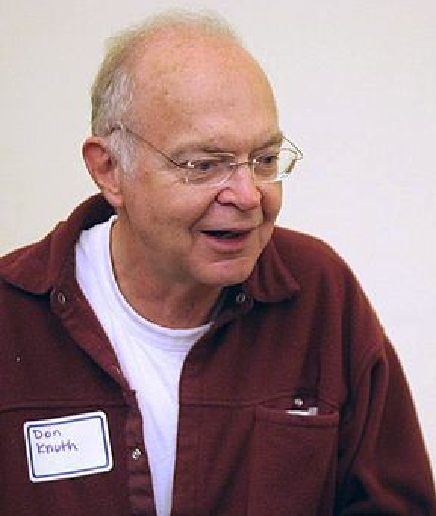
\includegraphics[height=4cm]{\freecalcBaseFolder/modules/freecalc-tutorial/pictures/DonaldKnuth.pdf} & 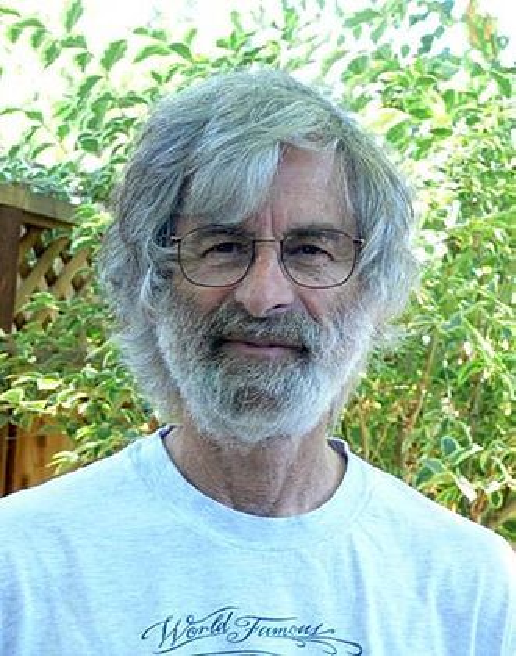
\includegraphics[height=4cm]{\freecalcBaseFolder/modules/freecalc-tutorial/pictures/LeslieLamport.pdf} \\
Donald Knuth & Leslie Lamport
\end{tabular}

\end{frame}